\documentclass[aps,pra, onecolumn,superscriptaddress,nopacs,floatfix, showkeys, notitlepage]{revtex4-1}
%   \documentclass[10pt]{article}



\usepackage{graphicx, color}
\usepackage{amssymb, amsmath}
\usepackage{times}
\usepackage[normalem]{ulem}
\usepackage{bbm}
\usepackage{todonotes}
\usepackage{mathtools}
\usepackage{enumitem} 
\usepackage{physics}
\usepackage{braket}
\usepackage{soul,xcolor}
\usepackage{subcaption}
\usepackage{bbold}
\usepackage{wrapfig}
\usepackage{multirow}

\usepackage{booktabs}  % for \toprule, \midrule, and \bottomrule macros 
\usepackage{tabularx}  % for 'tabularx' environment and 'X' column type
%\usepackage[hang,small,bf]{caption}
%\setlength{\captionmargin}{25pt}
%\usepackage{dblfloatfix}
\usepackage{tikz}
%%%<
\usepackage{verbatim}
%\usepackage[active,tightpage,floats]{preview}
%\PreviewEnvironment{tikzpicture}
%\setlength\PreviewBorder{5pt}%
%%%>
\usetikzlibrary{arrows}
\usetikzlibrary{positioning}
% Nice captions.
%\usepackage[hang,small,bf]{caption}
%\setlength{\captionmargin}{25pt}

% New commands to keep things tidy.
%\newcommand{\ket}[1]{$\left|#1\right\rangle$}
\newcommand{\Om}[1]{\small $\omega_{#1}$}
\newcommand{\De}[1]{$\Delta_{#1}$}
\newcommand{\Ga}[1]{$\Gamma_{#1}$}

%\newcommand{\Om}[1]{\small $\omega_{#1}$}
%\newcommand{\De}[1]{$\Delta_{#1}$}
%\newcommand{\Ga}[1]{$\Gamma_{#1}$}

\makeatletter
\newcommand*\bigcdot{\mathpalette\bigcdot@{.5}}
\newcommand*\bigcdot@[2]{\mathbin{\vcenter{\hbox{\scalebox{#2}{$\m@th#1\bullet$}}}}}
\newcommand*\cav{(\bigcdot)}
\newcommand*\ncav{(\bigcdot \bigcdot)}
\makeatother

%\newcommand{\ket}[1]{$\left|#1\right\rangle$}

\usepackage{amsmath}
\makeatletter
\def\env@cases{%
  \let\@ifnextchar\new@ifnextchar
  \left\lbrace
  \def\arraystretch{1.2}%
  \array{l@{\quad}l@{}}% Formerly @{}l@{\quad}l@{}
}



\begin{document}
\title{Note on temperature estimation}
\author{NanoQT}
\date{\today}

\begin{abstract}
Revisit the nanofiber temperature measurement scheme and incorporate the FBG dispersion.
In the current scheme, the temperature resolution of $\sim 40$ K is set by nanofiber length and we want to get finer resolution, i.e. $\delta T\sim 1$ K for monitoring and potentially preventing cavity degradation by appropriate cavity frequency measurement. Discuss the possibility of better resolution in temperature by using a 1D model of FBG.
%Also discuss the possibility of temperature measurement with chirped FBG cavity. 
\end{abstract}


\maketitle
%\tableofcontents

\section{Model: Temperature and frequency dependence}
To estimate the temperature of nanofiber by the cavity parameters, as described in Ref, \cite{Wuttke2013}, we consider a simple model: (1) the nanofiber is heated locally, leading to refractive index change $\delta n = \frac{\partial n}{\partial T}\delta T$ while the thermo elastic effect is negligible (one order magnitude smaller than thermo refractive one), (2) Fiber Bragg gratings add wavelength dependent phase shift due to the dispersion.  
%Note that we can safely ignore the wavelength dependence of Silica refractive index $\delta n/\delta \lambda=1.55\times 10^{-5}/$ nm @ 852.3 nm by using the Sellmeier formular since we are interested in small range of the wavelength.
Then, the round-trip phase shift in a cavity consists of propagation phase $\phi_\mathrm{nano}(T)$, $\phi_\mathrm{others}$ (\textit{nanofiber} regions and \textit{others} with the length of $L_\mathrm{nano}$ and $L_\mathrm{others}$, respectively) and dispersion of the FBGs $\phi_\mathrm{FBG}(\nu)$ as
\begin{eqnarray}
    \phi(\nu,T)&=&\phi_\mathrm{nano}(T)+\phi_\mathrm{others}+\phi_\mathrm{FBG}(\nu)\\
    &=&\frac{4\pi \nu n_\mathrm{nano}(T)L_\mathrm{nano}}{c}+\frac{4\pi \nu  n_\mathrm{ot} L_\mathrm{others}}{c}
    +\phi_\mathrm{FBG}(\nu)
\end{eqnarray}
where temperature of nanofiber region $T$.
For typical scan of 40 GHz (or 0.1 nm), the refractive index change of Silica is $\delta n = 1.55 \times 10^{-6}$. Then, a $m$-th cavity resonance is written by 
\begin{eqnarray}
 \phi(\nu_m)=2\pi m \quad\rightarrow\quad
    \nu_m &=& m\frac{c}{2 \mathcal{L}_\mathrm{cav}(\nu, T)}-\frac{c}{4\pi \mathcal{L}_\mathrm{cav}(\nu, T)}\phi_\mathrm{FBG}(\nu)\\
\mathrm{where}\quad    \mathcal{L}_\mathrm{cav}(T)  &=&n_\mathrm{nano}(T)L_\mathrm{nano}+n_\mathrm{ot} L_\mathrm{others}
\end{eqnarray}
where optical path length $\mathcal{L}_\mathrm{cav}$. 
The free spectral range is given by
\begin{eqnarray}
    \Delta_m\equiv\nu_m-\nu_{m-1}=
    \frac{c}{2\mathcal{L}_\mathrm{
cav}(\nu, T)}-\frac{c}{4\pi\mathcal{L}}\left(\phi_\mathrm{FBG}(\nu_m)-\phi_\mathrm{FBG}(\nu_{m-1})\right).
\end{eqnarray}
%is composed of a nanofiber and the rest of the sections, called, ``others''.
The small change in optical path length due to the temperature change $\delta T$ is approximated by
\begin{eqnarray}
        \delta \mathcal{L}_\mathrm{cav}(T)\approx \frac{\partial n_\mathrm{nano}}{\partial T} L_\mathrm{nano}\delta T 
\end{eqnarray}
%Note that thermo elastic term is ignored since the thermo-refractive coefficient is one order of magnitude larger.
Then, the change in a cavity resonance frequency $\delta \nu_m$ and the FSR $\delta \Delta_m$ (convenient observables) are given by 
\begin{eqnarray}
    \frac{\delta \nu_m}{\nu_m} &=&-\frac{L_\mathrm{nano}}{\mathcal{L}_\mathrm{cav}}\frac{\partial n_\mathrm{nano}}{\partial T}\delta T-\frac{c}{4\pi \mathcal{L}_\mathrm{cav}} \frac{\partial \phi_\mathrm{FBG}}{\partial \nu}\frac{\delta\nu}{\nu_m}
    \label{eq:df}
\\
    \frac{\delta\Delta_m}{\Delta_m} &=&-\frac{L_\mathrm{nano}}{\mathcal{L}_\mathrm{cav}}\frac{\partial n_\mathrm{nano}}{\partial T}\delta T-\frac{c}{4\pi \mathcal{L}_\mathrm{cav}} \left(\frac{\partial \phi_\mathrm{FBG}}{\partial \nu}\Big|_{\nu_{m}}-\frac{\partial \phi_\mathrm{FBG}}{\partial \nu}\Big|_{\nu_{m-1}}
    \right)\frac{\delta \nu}{\Delta_m}
%    &\approx&-1.4\times 10^{-7} \delta T-1.0\times 10^{-6}\frac{\partial \phi_\mathrm{FBG}}{\partial \nu}\delta \nu
\end{eqnarray}
These relations suggest that cavity resonance shift $\delta\nu_m$ is practically suited for measuring the temperature due to the higher carrier frequency of the signal and better suppression of the FBG contribution ($\delta\nu/\nu_m$ vs $\delta\nu/\Delta_m$).  
\textcolor{red}{[Corrected the $n_\mathrm{eff}$ dependence on the wavelength]} Note that the evaluation of $\partial n_\mathrm{nano}/\partial T$ is discussed in Appendix \ref{app:neff}.

For instance, we take typical settings of $dn_\mathrm{nano}/dT\approx 10^{-5}, L_\mathrm{nano}=1$ mm, $\nu_m= 351.7
$ THz (for Cs), and $ \mathcal{L}_\mathrm{cav}\sim n\cdot L_\mathrm{cav}$ with $n=1.454, \frac{\partial n_\mathrm{nano}}{\partial n}=0.72$ at $a=250$ nm (in Table \ref{tb:neff}), $L_\mathrm{cav}=5$ cm.
Then, the frequency shift is evaluated to be 
\begin{eqnarray}
    \frac{\delta \nu_m}{\nu_m} 
    \approx-9.9\times 10^{-6} \cdot\delta T-7.9\times 10^{-7}\cdot\frac{\partial \phi_\mathrm{FBG}}{\partial \nu}\delta \nu
    \label{eq:df_num}
\end{eqnarray}
Note that the nonlinear temperature dependence can be incorporated by using $\frac{\partial n}{\partial T}=9.6\times 10^{-6}+7.7\times 10^{-9}\cdot (T-299~\mathrm{K})$ as discussed in \cite{Wuttke2013, Wuttke_thesis}.



\subsection{Current scheme: Count cavity resonance numbers at the fixed frequency}
The current procedure is to keep track of number of drifted cavity resonance from $1$-to-$N$ FSR at the fixed frequency ($\delta\nu=0$), allowing us to estimate the temperature drift without an effect from the FBG dispersion. 
For instance,  by using Eq. (\ref{eq:df}), we obtain the case of 1 FSR shift $\Delta_m$ as,
\begin{eqnarray}
    \frac{\Delta_m}{\nu_m} =-\frac{L_\mathrm{nano}}{\mathcal{L}_\mathrm{cav}}\frac{\partial n_\mathrm{nano}}{\partial T}\delta T
     \quad\rightarrow\quad
    \delta T\approx\frac{\lambda}{2}\frac{1}{L_\mathrm{nano}\frac{\partial n_\mathrm{nano}}{\partial n}\frac{\partial n}{\partial T}}\sim 62~\mathrm{K}
\end{eqnarray}
where $\partial n_\mathrm{eff}/\partial n\approx 0.72$ at $\lambda=852$ nm and $a=250$ nm, $\partial n/\partial T=9.6\times 10^{-6}$, and  $L_\mathrm{nano}=1$ mm.


\subsection{Yb case: $d/\lambda<0.4$}
\begin{eqnarray}
    \delta T\approx\frac{\lambda}{2}\frac{1}{L_\mathrm{nano}\frac{\partial n_\mathrm{nano}}{\partial n}\left(\frac{\partial n}{\partial T}+\alpha\right)},\quad\mathrm{where}\quad\alpha=\frac{1}{L}\frac{\partial L}{\partial T}=5.5\times 10^{-7}
\end{eqnarray}


\begin{figure}[!h]  
    \centering
    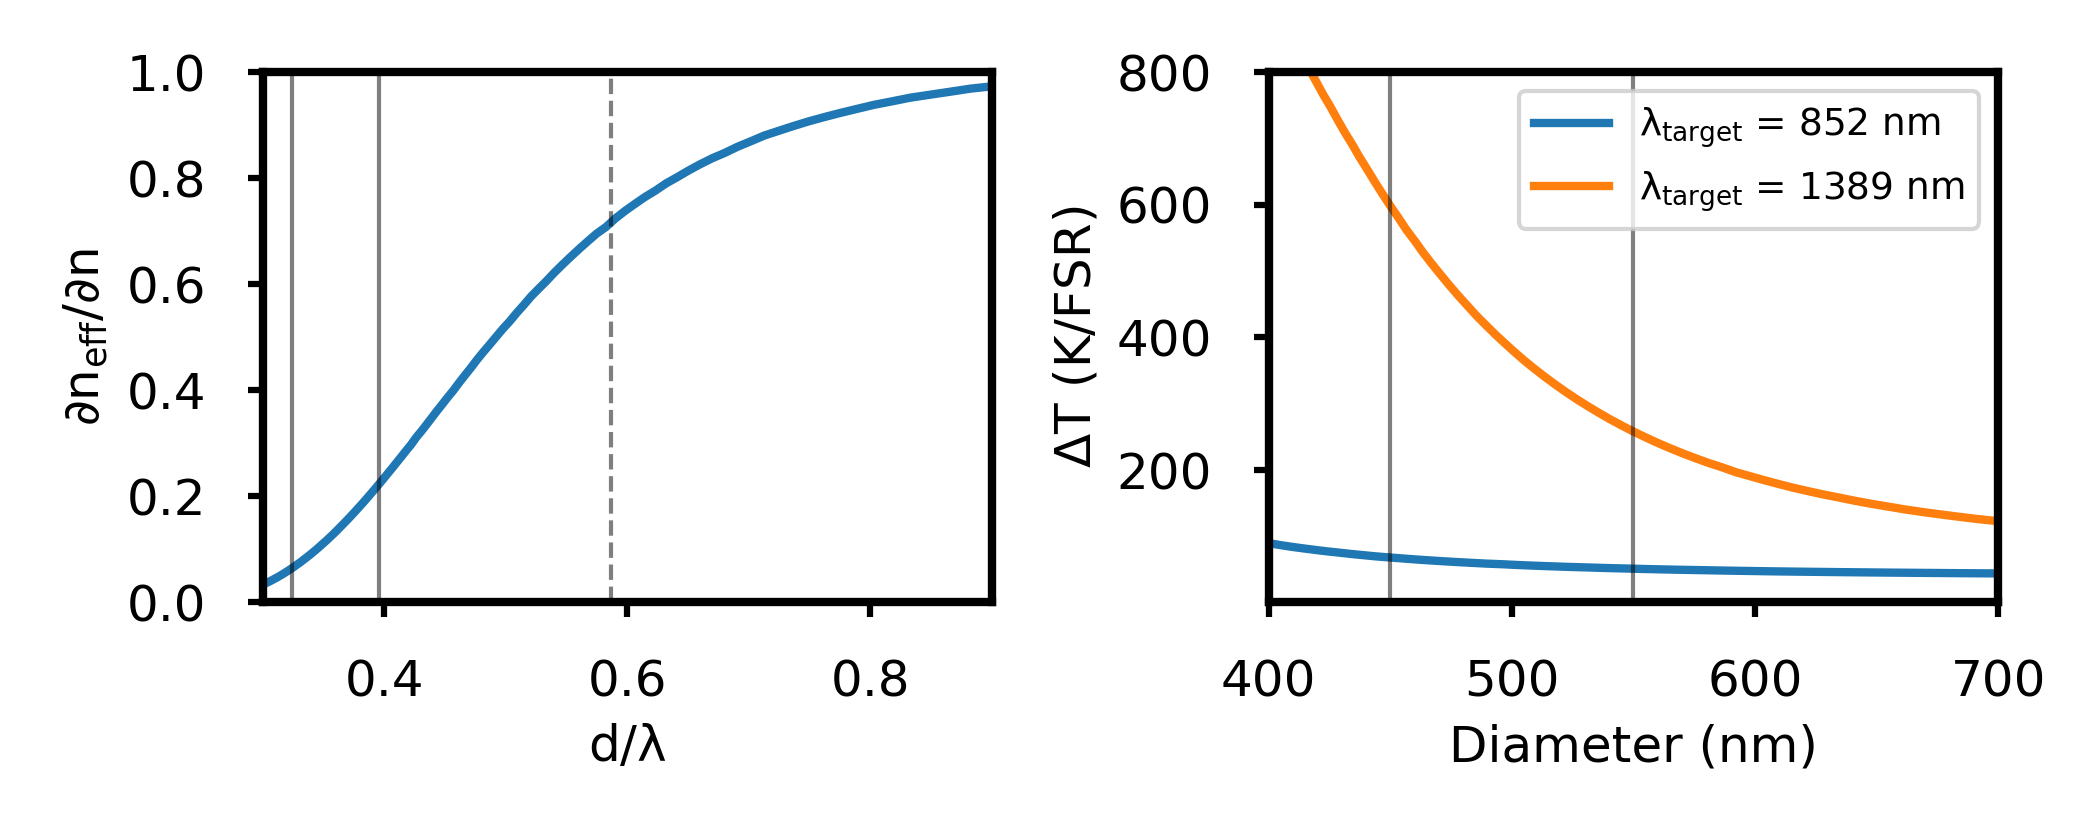
\includegraphics[width=0.65\linewidth]{fig/dneff_dn.png}
\caption{\textcolor{red}{[need update]} (left) Effective refractive index as a function fo the ratio of radius $a$ and $\lambda$. (right) Necessary temperature change to tune the cavity resonance by 1 FSR.}
\label{fig:tfsr}
\end{figure}

\subsection{Possibility of estimating temperature from cavity frequency change}
The goal is to obtain a sensitivity to $\delta T=1$ K, corresponding to 
$\frac{\delta \nu_m}{\nu_m}|_{\delta T}=-1.4\times 10^{-7}$ or $\delta \nu_m= 50$ MHz estimated by using Eq. (\ref{eq:df_num}).
Ideally, we want to suppress the contribution from FBGs by 1/10-th of thermorefractive one as
\begin{eqnarray}
\delta\phi_\mathrm{FBG}=\frac{\partial \phi_\mathrm{FBG}}{\partial \nu}\delta\nu=1.4\times 10^{-2}\quad \mathrm{(rad)}
\end{eqnarray}
By using the estimated value of $\frac{\partial \phi_\mathrm{FBG}}{\partial \nu}$ in Fig. \ref{fig:1dsim} (mimic a typical spectrum in the current system. See caption.) and assuming the symmetric cavity ($2\times \phi_\mathrm{FBG}$), we estimate the potential scanning range of frequency $\delta\nu$ as 
\begin{eqnarray}
    \mathrm{mid~gap:} &&\frac{\partial \phi_\mathrm{FBG}}{\partial \nu}\sim-0.037~\mathrm{rad/GHz~per~FBG}\quad\rightarrow\quad \delta \nu \sim 190~\mathrm{MHz}\\%\quad\leftrightarrow\quad \sim 8~\mathrm{K}\\
    \mathrm{near~bandedge:} &&\frac{\partial \phi_\mathrm{FBG}}{\partial \nu}\sim-0.1~\mathrm{rad/GHz~per~FBG}\quad\rightarrow\quad \delta \nu \sim 70~\mathrm{MHz}
\end{eqnarray}
Practically, one can dither the heating beam intensity and extract the power-to-temperature coefficient once every ten seconds or more, set by the free-running stability of the cavity. 

\begin{figure}[!h]  
        \centering
        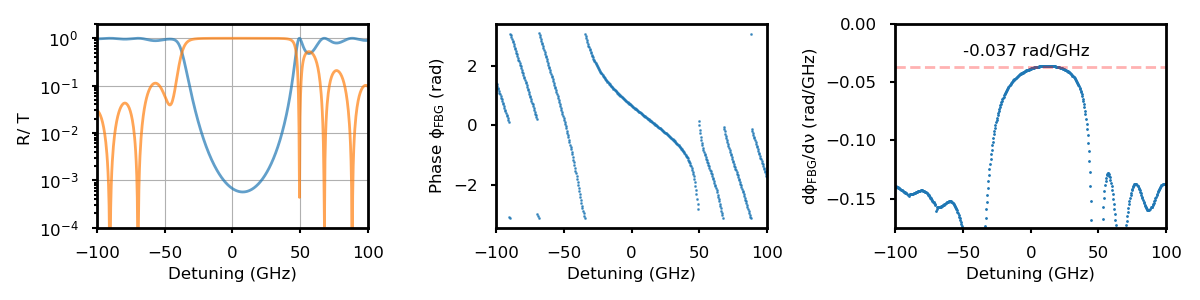
\includegraphics[width=1\linewidth]{fig/phase.png}
	\caption{Transmission/Reflection spectra and phase shift of a single FBG, estimated by a 1D model including the spatial inhomogenity of refractive index modulation $\delta n$. The inhomogenity is hand-picked by using a gaussian envelope with $\sigma=5$ mm and peak $\delta n = 3.6\times 10^{-4}$, leading to the asymmetry of the transmission/reflection spectra with respect to detuning (typically observed in the current system). The most right plot shows $\frac{\partial \phi_\mathrm{FBG}}{\partial}\sim-0.037$ rad/GHz at the mid gap
 %and $\frac{\partial \phi_\mathrm{FBG}}{\partial}\sim-0.1$ rad/GHz near the bandedge.
 }
    \label{fig:1dsim}
\end{figure}

\newpage


%\textcolor{red}{[brief discussion about diameter dependence]}



\appendix

\section{Fiber Bragg grating}
\subsection{1D model: uniformly alternate between $n$ and $n+\delta n$}
The FBG can be described by a 1D model with alternating two layers ($n_1, a_1)$ and $n_2, a_2)$. 
Analytical expressions of reflection and transmission coefficients are well know and convenient for later investigation as described in Ref. \cite{Bendickson1996}.
Here is a brief summary of key equations:
The transfer matrix of two layers ($n_1, a_1)$ and $n_2, a_2)$ is expressed by
\begin{eqnarray}
    M_{\mathrm{cell}}=\left(\begin{array}{cc}
1 / t^* & r / t \\
r^* / t^* & 1 / t
\end{array}\right)
\label{eq:tmat}
\end{eqnarray}
where $\phi_1=n_1 k a_1$, $\phi_2=n_2 k a_2$, and
\begin{eqnarray}
\frac{r}{t}  =\frac{i}{2}\left(\frac{-n_1}{n_2}+\frac{n_2}{n_1}\right) \sin \left(\phi_1\right) e^{-i\phi_2}, \quad
\frac{1}{t}  =\left(\cos \left(\phi_1\right)+\frac{i}{2}\left(\frac{n_1}{n_2}+\frac{n_2}{n_1}\right) \sin \left(\phi_1\right)\right) e^{i\phi_2}
\end{eqnarray}
The dispersion relation of an infinite 1D chain is given by using a unit cell length $a=a_1+a_2$ as
\begin{eqnarray}
%\mathrm{Tr}[M_\mathrm{cell}]&=&2\cos\beta a\\
    %\rightarrow
    \quad \cos (\beta a)&=&\cos \left(k n_1 a_1\right) \cos \left(k n_2 a_2\right)-\frac{1}{2}\left(\frac{n_1}{n_2}+\frac{n_2}{n_1}\right) \sin \left(k n_1 a_1\right) \sin \left(k n_2 a_2\right)
\end{eqnarray}
Then, $N$-periodic system is written by 
\begin{eqnarray}
    M_N=M_\mathrm{cell}^N = M_\mathrm{cell}\frac{\sin(N\beta a)}{\sin(\beta a)}-I\frac{\sin((N-1)\beta a)}{\sin(\beta a)}.
\end{eqnarray}
Thus, transmission and reflection coefficient is written by \cite{Bendickson1996}
\begin{eqnarray}
    \frac{r_N}{t_N}=\frac{r}{t}\frac{\sin(N\beta a)}{\sin(\beta a)}, \quad
    \frac{1}{t_N}=\frac{1}{t}\frac{\sin(N\beta a)}{\sin(\beta a)}-\frac{\sin((N-1)\beta a)}{\sin(\beta a)}
\end{eqnarray}
As shown in Fig. \ref{fig:dn_dep}, the larger bandgap ($\propto \delta n/n$) leads to the smaller $\partial \phi_\mathrm{FBG}/\partial T$.
%Note that the quarter-wave stack model is convenient to derive a compact form of $R/T$ and phase as shown in Ref. \cite{Bendickson1996}.
\begin{figure}[!h]  
        \centering
        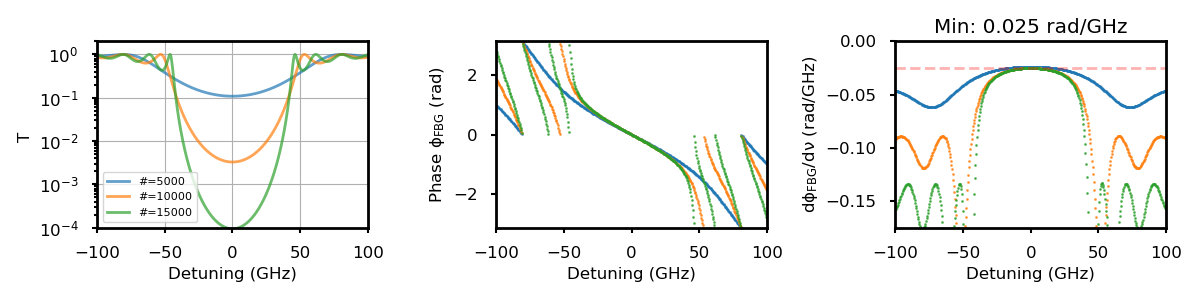
\includegraphics[width=1\linewidth]{fig/phase_21_20_17.png}
	\caption{Cell number dependence of uniform FBG with $\delta n/n=3.6\times 10^{-4}$: $N_\mathrm{cell}=5000, 10000, 15000$, corresponding to FBG length of $1.8$ mm, 3.6 mm and 5.3 mm, respectively. At the center of the bandgap, $d\phi_\mathrm{FBG}/d\nu = -0.025$ rad/GHz, independent of the cell number.}
    \label{fig:ncell_dep}
\end{figure}

\begin{figure}[!h]  
        \centering
        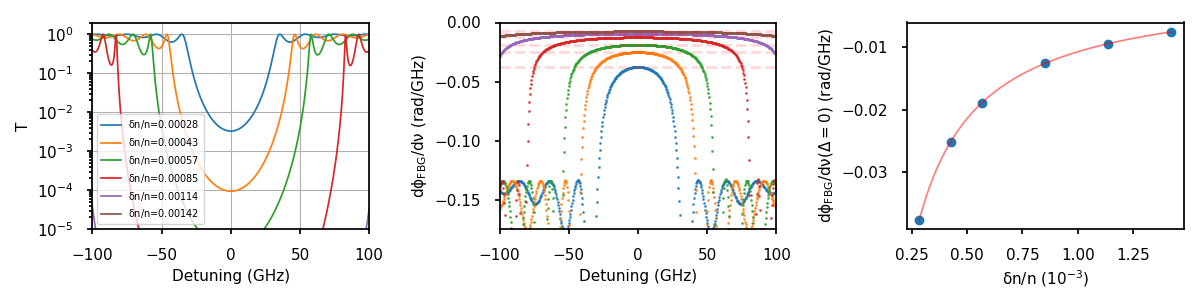
\includegraphics[width=1\linewidth]{fig/phase_22_17_23_25_26_24.png}
	\caption{Modulation $\delta n$ dependence with $N_\mathrm{cell}=15000$: As increasing the modulation amplitude $\delta n$, the band gap increases owing to $\Delta\nu_\mathrm{gap}/\nu=\delta n/n$. As a result, the slope the phase shift approaches to zero with a asymptotic form of $\frac{\partial \phi_\mathrm{FBG}}{\partial \nu} = \frac{A}{1+(\delta n/n)/B}$ where $A=-11.2(2.0), B=9.5(1.7)\times 10^{-7}$.}
    \label{fig:dn_dep}
\end{figure}
\vspace{-7mm}
\subsection{1D model: gaussian envelope of $\delta n$}
Using the transfer matrix of Eq. (\ref{eq:tmat}) with spatially dependent $\delta n$ (gaussian distribution with $\sigma = 5$ mm, N=15000), we numerically compute the $\tilde{M}_N = \prod_i^N M_\mathrm{cell}(\delta n_i)$ as shown in Fig. \ref{fig:1dsim}

\section{1D model of FBG cavity:Relation between mirror phase shift and change in cavity FSR}
Considering a FBG cavity with active region $L$ withou taper regions as in Ref. \cite{Barmenkov2006},  the free spectral range of the cavity and location of cavity resonance are approximated by
\begin{eqnarray}
    \nu_m &\approx& \Delta_{0}\left(m-\frac{\phi_\mathrm{FBG}(m\cdot \Delta_{0})}{2\pi}\right)\\
    \Delta_{m}&\approx &\Delta_{0}\left(1-\frac{1}{2\pi}\frac{\partial \phi_\mathrm{FBG}}{\partial \nu}\Delta_{0}\right),\quad\mathrm{where}\quad \Delta_{0}=\frac{c}{2n_\mathrm{eff}L}
\end{eqnarray}
Note $\phi_\mathrm{FBG}$ should incorporate the phase shift of two FBGs.
Add comparison of projected FSR and transfer matrix calculation.

As described in Ref. \cite{Barmenkov2006}, 

\begin{figure}[!h]  
        \centering
        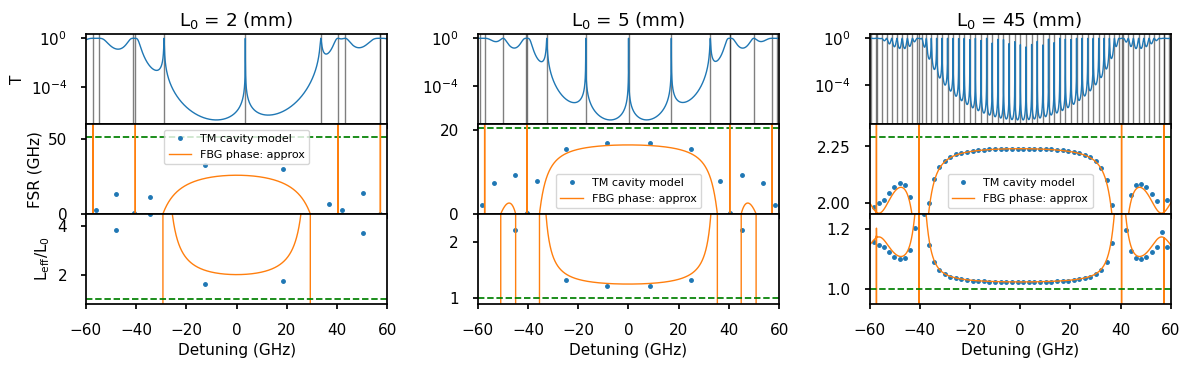
\includegraphics[width=1\linewidth]{fig/disperson.png}
	\caption{Cell number dependence of uniform FBG with $\delta n/n=4.3\times 10^{-4}$: $N_\mathrm{cell}=15000$, corresponding to FBG length of $4.4$ mm, respectively. Length between FBG regions, (left) $L_0=2$ mm, (middle) $5$ mm (right) $45$ mm, corresponding FSR of $0.5$, $2.3$ and $50$ GHz, respectively.}
    \label{fig:ncell_dep}
\end{figure}


\subsection{Cavity frequency shift due to the temperature change of FBG}
When heating one of the FBGs, the sensitivity to the frequency shift per single FBG is given by
\begin{eqnarray}
    \frac{\partial \nu_m}{\partial T}&\approx& \nu_B\cdot \left(\frac{1}{n}\frac{\partial n}{\partial T}\right)\cdot \left(\frac{\Delta_0}{2\pi}\frac{\partial \phi_\mathrm{FBG}(\nu)}{\partial \nu}\right)\\
    &\sim & 1100\cdot \left(\frac{\partial \phi_\mathrm{FBG}/\partial \nu}{1.0 ~\mathrm{[rad/GHz]}}\right) ~[\mathrm{MHz/K}]
\end{eqnarray}
where thermo-refractive coefficient $\frac{1}{n}\frac{\partial n}{\partial T}=8.6\times 10^{-6}$ at 300 K  and FSR of the cavity $\Delta_0=2.3$ GHz.
At the region of interest, from the bottom of the stopband to the edge, this coefficient ranges $\frac{\partial \nu_m}{\partial T}\sim 10-100$ MHz/K. 

\subsection{Tuning external coupling rate}
\begin{eqnarray}
    \kappa_\mathrm{ex}(\nu)&=&\frac{1}{2}\Delta_m T_\mathrm{FBG}(\nu)\\
    \frac{\partial\kappa_\mathrm{ex} }{\partial T}&=& 
        =\left(\frac{\partial \nu}{\partial T}\right) \cdot \left(\frac{\partial \kappa_\mathrm{ex}}{\partial \nu}\right)\approx\left(\frac{\nu_B}{n}\frac{\partial n}{\partial T}\right) \cdot \left(\frac{\partial \kappa_\mathrm{ex}}{\partial \nu}\right)\quad \mathrm{where}\quad \nu_B=2n\Lambda
\end{eqnarray}
\begin{figure}[!h]  
        \centering
        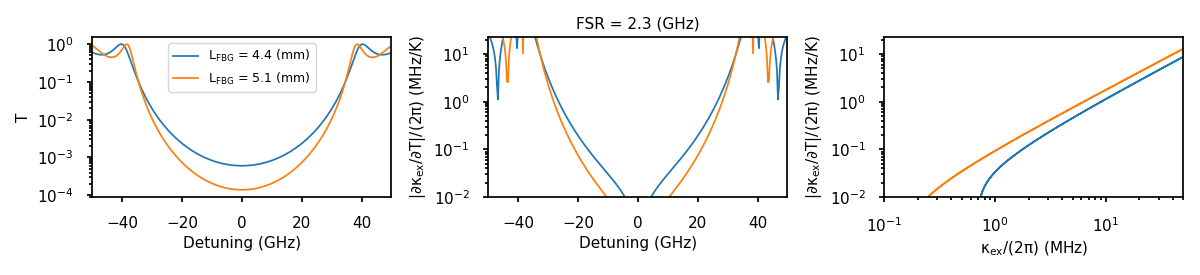
\includegraphics[width=1\linewidth]{fig/FBG_tuning.png}
	\caption{Cell number dependence of uniform FBG with $\delta n/n=4.3\times 10^{-4}$: $N_\mathrm{cell}=15000$, corresponding to FBG length of $4.4$ mm, respectively. Length between FBG regions, (left) $L_0=2$ mm, (middle) $5$ mm (right) $45$ mm, corresponding FSR of $0.5$, $2.3$ and $50$ GHz, respectively.}
    \label{fig:fbgtuning}
\end{figure}


\begin{figure}[!h]  
        \centering
        
\includegraphics[width=1\linewidth]{fig/FBG_tuning_nonuni.png}
	\caption{plot $\partial \kappa_\mathrm{ex}/\partial T$ vs $\kappa_\mathrm{ex}$.}
    \label{fig:fbgtuningGaussian}
\end{figure}


\section{Evaluation of effective index sensitivity $\partial n_\mathrm{nano}/\partial n$}
\label{app:neff}
The temperature dependence phase shift is given by the effective index of the nanofiber $n_\mathrm{eff}(T)$ as
\begin{eqnarray}
    \phi(\nu, T)=2 k_0 n_\mathrm{nano}(T)\,L_\mathrm{nano}\quad\rightarrow\quad \delta \phi(\nu, T)=2 k_0 L_\mathrm{nano}\frac{\partial n_\mathrm{nano}}{\partial n}\frac{\partial n}{\partial T}\delta T_\mathrm{nano}
\end{eqnarray}
In the Table \ref{tb:neff}, we evaluated several configurations.
\begin{table}[h]
\centering
\begin{tabular}{|c|c|c|}
\hline
$\lambda$ (nm) & Radius (nm) & $\partial n_{\mathrm{eff}}/\partial n$ \\
\hline
852  & 250 & 0.72  \\
\hline
1389 & 325 & 0.42  \\
1389 & 275 & 0.22  \\
1389 & 225 & 0.063 \\
\hline
\end{tabular}
\caption{Effective index sensitivity $\partial n_{\mathrm{eff}}/\partial n$ for different wavelengths $\lambda$ and fiber radii $a$.}
\label{tb:neff}
\end{table}


\iffalse

\section{(WIP) BBR Stark Shift Estimates for the Yb Clock transition}
Here we quantify the black-body radiation (BBR) Stark shifts for the neutral-Yb optical clock transition
\({}^{1}S_{0}\leftrightarrow {}^{3}P_{0}\), and estimate local BBR contributions from a nearby hot cylindrical object (e.g.\ a nanofiber) at temperature $T$.

{\bf BBR Electric Field}: The rms electric field due to isotropic BBR at temperature $T$ is
\begin{equation}
E_\mathrm{rms}(T) = 831.945~\mathrm{V/m}\,\left(\frac{T}{300~\mathrm{K}}\right)^{2}, \qquad
\langle E^{2}\rangle_{T} = E_\mathrm{rms}^{2} \propto T^{4}.
\end{equation}

{\bf BBR Stark Shift}: For a clock state $\lvert i\rangle\in\{g~(^{1}S_{0}),\,e~(^{3}P_{0})\}$ with static scalar polarizability $\alpha_i(0)$ \cite{Porsev2006},
\begin{eqnarray}
    \Delta\nu_i(T) = -\frac{1}{2h}\,\alpha_i(0)\,\langle E^{2}\rangle_{T}\,\bigl[1+\eta_i(T)\bigr].
\end{eqnarray}
where $\eta_i(T)$ is a dynamic correction. 
If $\alpha_i(0)$ is expressed in atomic units (1~a.u. $=1.648777274\times10^{-41}\,\mathrm{C\cdot m^{2}/V}$),
\begin{equation}
\Delta\nu_i(T)\,[\mathrm{Hz}] = -\,0.00861123\ \alpha_i[\mathrm{a.u.}] \left(\frac{T}{300~\mathrm{K}}\right)^{4} \left[1+\eta_i(T)\right].
\end{equation}

{\bf Clock (Differential) Shift}:
The clock shift is given by
\begin{equation}
\Delta\nu_\text{clock}(T) = \Delta\nu_{e}(T)-\Delta\nu_{g}(T)
= -\,0.00861123\ \Delta\alpha(0)\,
\left(\frac{T}{300~\mathrm{K}}\right)^{4} \left[1+\eta_\text{clock}(T)\right],
\end{equation}
with $\Delta\alpha(0)=\alpha_{e}(0)-\alpha_{g}(0)$ and
\begin{equation}
\eta_\text{clock}(T) = \frac{\alpha_{e}(0)\eta_{e}(T)-\alpha_{g}(0)\eta_{g}(T)}{\Delta\alpha(0)}.
\end{equation}

{\bf Dynamic Correction}:
The dynamic correction $\eta_i(T)$ can be defined via the Planck-weighted integral over $\alpha_i(\omega)$.  
A rapidly convergent expansion valid when $\hbar\omega_{ki}\gg k_BT$ is
\begin{equation}
\eta_i(T) \approx \frac{80\pi^{2}}{63}\left(\frac{k_BT}{\hbar}\right)^{2}\frac{C_{2}^{(i)}}{\alpha_i(0)} \;+\;
\frac{16\pi^{4}}{15}\left(\frac{k_BT}{\hbar}\right)^{4}\frac{C_{4}^{(i)}}{\alpha_i(0)}+\cdots,
\end{equation}
with Cauchy moments
\begin{equation}
C^{(i)}_{2n} = \frac{2}{3\hbar}\sum_k \frac{|\langle k\Vert\mathbf d\Vert i\rangle|^{2}}{\omega_{ki}^{\,2n+1}}.
\end{equation}
For Yb near 300~K, $\eta_\text{clock}\sim +1.4\%$ and scales approximately as $\propto T^{2}$.

{\bf Adopted Polarizabilities}:
$\alpha_g(0)\approx 139~\mathrm{a.u.}$, $\alpha_e(0)\approx 285~\mathrm{a.u.}$, hence $\Delta\alpha(0)\approx 146~\mathrm{a.u.}$ \cite{Beloy2012}.  
This yields a static differential shift of $\approx -1.26$~Hz at 300~K; with $\eta_\text{clock}\approx 1.4\%$, the corrected value is $\approx -1.28$~Hz.

\begin{table}[h!]
\centering
\caption{Static (DC) scalar polarizabilities of the Yb clock states \cite{Beloy2012}. 
Values are given in atomic units (a.u.).}
\begin{tabular}{c c}
\hline
State & Polarizability $\alpha(0)$ (a.u.) \\
\hline
Ground state ${}^{1}S_{0}$ & $139$ \\
Excited state ${}^{3}P_{0}$ & $285$ \\
\hline
Differential $\Delta\alpha(0)$ & $146$ \\
\hline
\end{tabular}
\end{table}


\begin{table}[h!]
\centering
\caption{Estimated BBR Stark shifts of Yb clock states and transition frequency. 
Polarizabilities from Beloy (2012) midpoints. Dynamic correction 
$\eta_\text{clock}$ applied as described in the text. The last column gives the
clock shift for a hemisphere at temperature $T$ (other hemisphere cold), i.e.\ half of the full-sphere value.}
\begin{tabular}{c c c c | c}
\hline
Temperature & Ground state (${}^{1}S_{0}$) & Excited state (${}^{3}P_{0}$) & Differential (clock) & [Hemisphere] Differential (clock) \\
$T$ (K) & $\Delta\nu_g$ (Hz) & $\Delta\nu_e$ (Hz) & $\Delta\nu_{\text{clock}}$ (Hz) & $\Delta\nu_{\text{clock,hemi}}$ (Hz) \\
\hline
300 & $-1.22$ & $-2.48$ & $-1.28$ & $-0.64$ \\
330 & $-1.79$ & $-3.64$ & $-1.88$ & $-0.94$ \\
400 & $-3.46$ & $-7.03$ & $-3.63$ & $-1.815$ \\
600 & $-19.2$ & $-39.0$ & $-20.1$ & $-10.05$ \\
\hline
\end{tabular}
\end{table}



{\bf Local Hot Cylinder (Infinite-Length Model)}
For a cylinder of radius $r=d/2$ at distance $x$ from its surface (so that the atom--axis distance is $R=x+r$), a view-factor proxy for the fractional solid angle is
\begin{equation}
f \equiv \frac{\Omega}{4\pi}\;\approx\;\frac{\arcsin(r/R)}{\pi}, \quad (r\ll R).
\end{equation}
The effective rms field contribution is
\begin{equation}
E_\text{eff} = \sqrt{f}\,E_\mathrm{rms}(T),
\end{equation}
and the induced clock shift scales with $f$.  
Example: for $d=500\,\mathrm{nm}$ and $x=100\,\mu\mathrm{m}$, $f\approx 7.9\times10^{-4}$; at 300~K, $E_\text{eff}\approx 23~\mathrm{V/m}$, giving a clock shift $\sim 10^{-3}$~Hz.  
Increasing $x$ to 300~$\mu$m reduces this by a factor $\sim 3$ in field and $\sim 9$ in shift.


\subsection{Static Polarizabilities of Yb: Implication to ${}^3\mathrm{D}_1$}
The static (DC) dipole polarizability of an atomic state $|0\rangle$ is given by second-order perturbation theory as
\begin{equation}
    \alpha(0) = \frac{2}{3\hbar}\sum_k \frac{|\langle k \| \mathbf{d} \| 0 \rangle|^2}{\omega_{k0}},
\end{equation}
where the sum runs over all opposite-parity excited states $|k\rangle$, $\omega_{k0} = (E_k - E_0)/\hbar$ is the transition angular frequency, and $\langle k \| \mathbf{d} \| 0 \rangle$ is the reduced dipole matrix element. The static polarizability thus reflects a weighted sum of oscillator strengths divided by transition energies. 

{\bf Major contributions}: In practice, the dominant contributions arise from the lowest-lying dipole-allowed transitions. For ytterbium:
\begin{itemize}
    \item The ground state $^1S_0$ polarizability is primarily determined by the strong $^1S_0 \rightarrow {}^1P_1$ resonance transition at 399~nm.
    \item For the clock excited state $^3P_0$, the leading contributions come from nearby $^3D_1$, $^3S_1$, and higher triplet states.
    \item For the metastable $^3D_1$ state, opposite-parity $^3P$ and $^3F$ states provide the strongest contributions.
\end{itemize}
Because the dominant optical transitions in Yb lie in the near-UV to visible spectral range (photon energies of a few eV) and electric dipole matrix elements are typically a few atomic units, the resulting static polarizabilities are of order $10^2$ atomic units (a.u.). 
For reference:
\begin{align}
    \alpha_{^1S_0}(0) &\approx 139~\mathrm{a.u.}, \\
    \alpha_{^3P_0}(0) &\approx 285~\mathrm{a.u.}, \\
    \alpha_{^3D_1}(0) &\sim \text{a few}~10^2~\mathrm{a.u.},
\end{align}
as reported by Beloy~\cite{Beloy2012} and subsequent theoretical works. Metastable triplet states typically exhibit larger polarizabilities than the ground singlet state, owing to their smaller energy separations to nearby opposite-parity levels.

{\bf Implications for BBR shifts}: For blackbody radiation shifts, the static approximation is usually adequate, since the BBR spectrum at 300~K peaks near 6~THz, far below optical transition frequencies.
However, in Yb the proximity of the $^3P_0 \rightarrow {}^3D_1$ transition at 1389~nm enhances the frequency dependence, requiring the introduction of a dynamic correction $\eta(T)$, typically of order $1$--$2\%$ at room temperature.

\section{(WIP) BBR vs Radiation from nanofiber}

\fi

\bibliography{mybib} 



\end{document}
